\documentclass[onecolumn, 11pt, hmargin=1in, vmargin=1in]{aastex62}
%%%%%%begin preamble
\usepackage{hyperref}
\usepackage{url}
\usepackage{natbib}
\setlength{\bibsep}{0pt plus 0.3ex}
\usepackage{graphicx}
\usepackage{amsmath}
\usepackage{amssymb}

\usepackage{color}
\hypersetup{
  colorlinks   = true,
  %citecolor    = blue
  citecolor    = gray
  % gray is not being found!?!
  % gray is found if pdfpages is used... crap.
  %citecolor    = grey
  %citecolor    = Gray
}

%Copy+pasted from aastex.
\newcommand\prf{Phys.~Rev.~Fluids}     % Astrophysical Journal, Letters 
%% headers
\usepackage{fancyhdr}
\pagestyle{fancy}
\fancyhf{} % sets both header and footer to nothing
\lhead{Evan Anders---Research Statement}
\rhead{Stanford University, Stanford Science Fellows}
\cfoot{\footnotesize{\thepage}}
%\pagestyle{empty}
%\pagenumbering{gobble}
%\renewcommand*{\thefootnote}{\fnsymbol{footnote}}

\renewcommand{\vec}{\ensuremath{\boldsymbol}}
\newcommand{\dedalus}{\href{http://dedalus-project.org}{Dedalus}}
\newcommand{\del}{\ensuremath{\vec{\nabla}}}
\newcommand{\scrS}{\ensuremath{\mathcal{S}}}


%\usepackage{atbegshi}
%%%%%%end preamble


\begin{document}
\section*{}
\thispagestyle{fancy}

\begin{center}
\vspace{-1in}
\textbf{Motivation and Research Problem: The Solar Convective Conundrum}
\vspace{-8pt}
\end{center}

Stars are the cornerstone of studies in astrophysics and are themselves fascinating experiments where fluid dynamical processes occur at extreme parameters.
The relatively new field of asteroseismology measures wavelike deformations along stellar surfaces and uses those measurements to learn about the structure of stellar interiors.
Asteroseismology can precisely determine the age, mass, and radius of Sun-like stars, and these measurements are used broadly across astrophysical disciplines like exoplanetary science and galactic archaeology \citep{huber&all2019}.
The interpretation of asteroseismic data relies on 1D models of stellar interiors.
Stars like the Sun have convection zones near their surfaces, but turbulent 3D processes like convection are handled using decades-old parameterizations \citep[e.g.,][]{bohm-vitense1958} in the creation of these 1D models.
These parameterizations predict that ``giant cells'' characterized by massive horizontal motions should be driven deep in those convective regions, but giant cells are absent in observations of the Sun \citep{hanasoge&all2015}.
The absence of giant cells is called the ``Solar Convective Conundrum'' and implies that our most fundamental understanding of convection in stars is incomplete.
Solving this Convective Conundrum---which in turn will improve stellar models and broadly-used asteroseismic measurements---is crucial.



\begin{center}
\vspace{-5pt}
\textbf{Research Plan: Stellar Convection Across Spatial Scales}
\vspace{-8pt}
\end{center}
\begin{figure*}[b]
	\begin{center}
	\vspace{-8pt}
    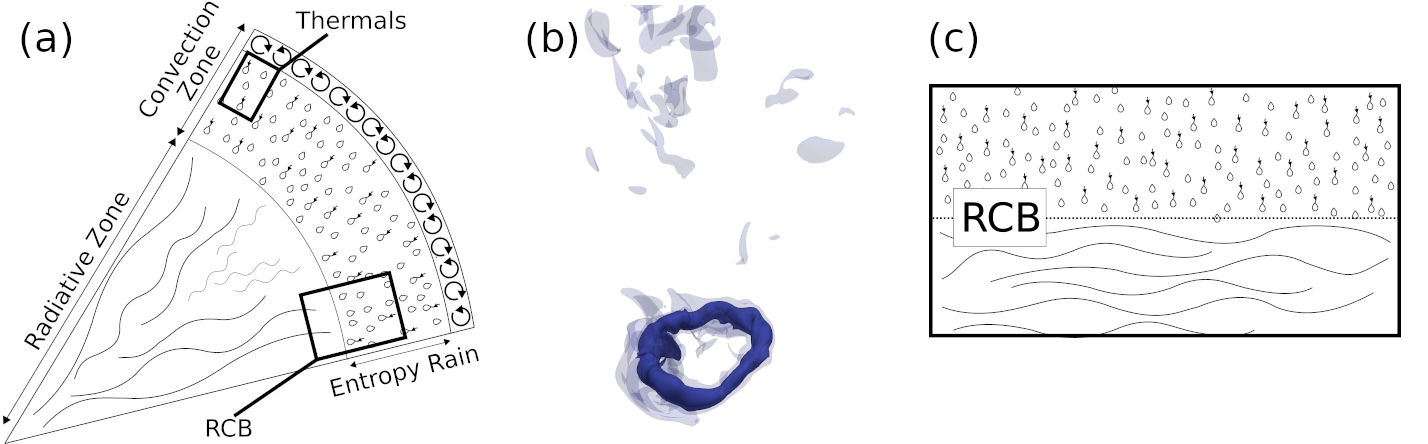
\includegraphics[width=0.95\textwidth]{./figs/tri_panel.png}
	\vspace{-8pt}
    \caption{ 
	(a) A schematic of the interior of Sun-like stars under the entropy rain hypothesis, where cold droplets of fluid carry the stellar luminosity below a small traditional convective surface layer.
	The scope of two experiments proposed here are boxed and labeled (``Thermals'' and ``RCB''), and the third experiment proposed here would contain the full spherical volume of the star, from which this wedge is taken.
	(b) A 3D visualization of entropy perturbations within the downward-propagating reference frame of a turbulent ``thermal,'' which models a stellar downflow.
	(c) A schematic of the radiative-convective boundary (RCB), where downflows impinge upon a stable layer and excite gravity waves within that layer.
	\label{fig:tri_panel} }
	\end{center}
\end{figure*}


Modern convective simulations reliably reproduce flows at the Sun's surface; however, simulations of deep convection often disagree with modern observations and drive giant cells.
During my time at Stanford, I will conduct a series of studies, outlined in Fig.~\ref{fig:tri_panel}, which span from the smallest to the largest scales in stellar convection.
%I will progressively build on understanding gained in detailed small scale studies to inform studies which focus on increasingly larger scales.
I will carry out my simulations using the Dedalus code \citep{burns&all2019}, which I have used throughout my PhD research.

Stratified convection, such as in the Sun's convection zone, exhibits broad slow upwellings in balance with intense, fast downflows.
The ``entropy rain'' hypothesis posits that downflows alone are powerful enough to transport the Sun's luminosity deep in the convection zone (see Fig.~\ref{fig:tri_panel}a).
This hypothesis is gaining traction \citep{brandenburg2016, kapyla&all2017} and could explain the absence of giant cells in observations \citep{hanasoge&all2015}.

Regardless of the veracity of the entropy rain hypothesis, the nature of downflows in solar convection and their deep interactions must be better understood.
As a Stanford fellow, I will spend my first two years studying solar downflows to help clarify the convective conundrum.
These downflows may turbulently break up into distinct pieces as they fall and these individual downflow pieces can be modeled as ``thermals'' (a turbulent evolved thermal is visualized in Fig.~\ref{fig:tri_panel}b).
Thermals are studied extensively in Earth's atmosphere \citep{lecoanet&jeevanjee2019} and I recently studied them in the solar context \citep{andersLB2019}.
In my first year as a fellow, I will study thermals-as-downflows to understand how the Sun's magnetism and global rotation affect the propagation of individual downflows.
I will constrain whether magnetic Lorentz or rotational Coriolis forces in the Sun can prevent downflows from transiting the full solar convection zone to help determine the plausibility of the entropy rain hypothesis.

After examining individual downflows, I will spend my second year examining interactions between downflows and the base of the solar convection zone, as in Fig.~\ref{fig:tri_panel}c.
The base of the convection zone in Sun-like stars is a radiative-convective boundary (RCB), where the turbulent convection zone meets a stably stratified ``radiative zone'' where radiation effectively carries the stellar luminosity.
I will build on my PhD convection work \citep{anders&brown2017, anders&all2019} and recent RCB work \citep{wood&brummell2018} to study the mechanisms through which an ensemble of downflows interacts with the RCB.
I will learn how downflows pump energy, magnetic fields, and angular momentum into the radiative zone.
Parameterizations predict that giant cells should be driven near the RCB, but mixing of near-RCB fluid by downflows may stabilize the deep convection zone and prevent the acceleration of giant cell flows.
Furthermore, the topology of a star's magnetic field and angular momentum profile can affect asteroseismic measurements \citep{benomar&all2018, santos&all2018}.
Pumping of magnetism and angular momentum into the RCB is poorly understood, but is crucial in establishing the topology of these fields.

In my third year as a fellow, I will examine spherical global simulations of Suns (Fig.~\ref{fig:tri_panel}a is a schematic of a wedge of such a simulation).
Recently, \citet{jorgensen&weiss2019} improved 1D stellar structure models by coupling them with 3D simulations of convection in thin, near-surface layers.
This coupling cannot be done generically for 3D simulations of \emph{deep}, turbulent convective motions because the timescale of atmospheric equilibration is very long compared to the size of timesteps required to resolve flows.
It is very computationally expensive to create a single equilibrated solution through standard timestepping techniques, so creating equilibrated solutions for arbitrary stars is impossible.
In \citet{anders&all2018}, I developed a mechanism which rapidly equilibrates simple Cartesian convection simulations (requiring e.g., an order of magnitude fewer cpu-hours than traditional techniques).
During my time at Stanford, I will extend this work to design, validate, and publicly release a generalized module which rapidly equilibrates the atmospheric structure and mean fluid flows in 3D global simulations.
This tool will allow for the efficient production of global simulations with deep convection from which convective statistics can be sampled to improve stellar models, as in \citet{jorgensen&weiss2019}.
I will personally employ this tool to equilibrate global simulations where I will examine downflows and RCB interactions.
I will compare these simulations to my previous two years' work to elucidate why modern observations and global simulations disagree so strongly about giant cells.


\begin{center}
\vspace{-5pt}
\textbf{How Stanford Enables These Accomplishments}
\vspace{-8pt}
\end{center}
Stanford is the perfect location for carrying out this work due to the opportunities available for interdisciplinary collaboration between astrophysicists, geophysical fluid dynamicists, applied mathematicians, and turbulence experts.
Prof.~Tom Abel of Stanford's physics department is the most natural collaborator for this work due to his expertise in astrophysical fluid dynamics and scientific visualization, as well as his broad interest in astrophysical topics.
From Prof.~Abel's group, I would collaborate with the numerous experts in Stanford's Physics department, such as Prof.~Petrosian, who has recently studied the hydrodynamics of solar flares and Prof.~Wagoner, who has studied waves in astrophysical accretion disks.
There are many other natural collaborators with expertise in fluid dynamics across Stanford, such as Profs.~Sheshadri and Thomas in the Dept.~of Earth System Science and Profs.~Ryzhik and Tokieda in the Mathematics Department.
Stanford's Center for Turbulence Research, with experts in turbulent fluid dynamics like Prof.~Jim\'{e}nez, will also be an invaluable resource as I carry out my research plan.
The computational requirements of this work are modest, and the resources available through Stanford's Research Computing Center, including the Sherlock HPC cluster, far exceed what will be required to complete this work.

The Stanford Science Fellows program would give me the freedom to study these ambitious problems in astrophysical fluid dynamics.
The projects proposed here seek to understand stellar convection from small to global scales, build naturally upon my PhD research, and help solve exciting problems in stellar structure with applications across astrophysics.
I look forward to the opportunity to create cross-disciplinary collaborations and carry on Stanford's excellent research tradition while making lasting contributions which help solve the Convective Conundrum.

\vspace{-11pt}
\bibliographystyle{yahapj}
\bibliography{biblio}
\end{document}
